\section{Clustering und Ausreißer}
\label{sec:clustering}

\paragraph{Räumliche Indexstrukturen --- Motivation}
\begin{itemize}
	\item Was ist die nächste Bar, die mein bevorzugtes Bier ausschenkt?
	\item \textbf{Bereichsanfrage}: Wie viele Restaurants gibt es im Stadtzentrum?
	\item Ähnlichkeitssuche Bilder: Distanz im Merkmalsraum = Maß der Unähnlichkeit
	\item Ziel eines \textbf{Index}: Zahl der zu ladenden Seiten minimieren
\end{itemize}

\paragraph{Index --- B+-tree}
\begin{itemize}
	\item = non-clustered primary B+-tree
	\item Beispiel: Student(name, age, gpa, major), B+T für gpa \\* (kleiner=links, größer=rechts, (gpa, (Seite, Eintrag)))
	\begin{figure}[H]\centering\label{BPTree}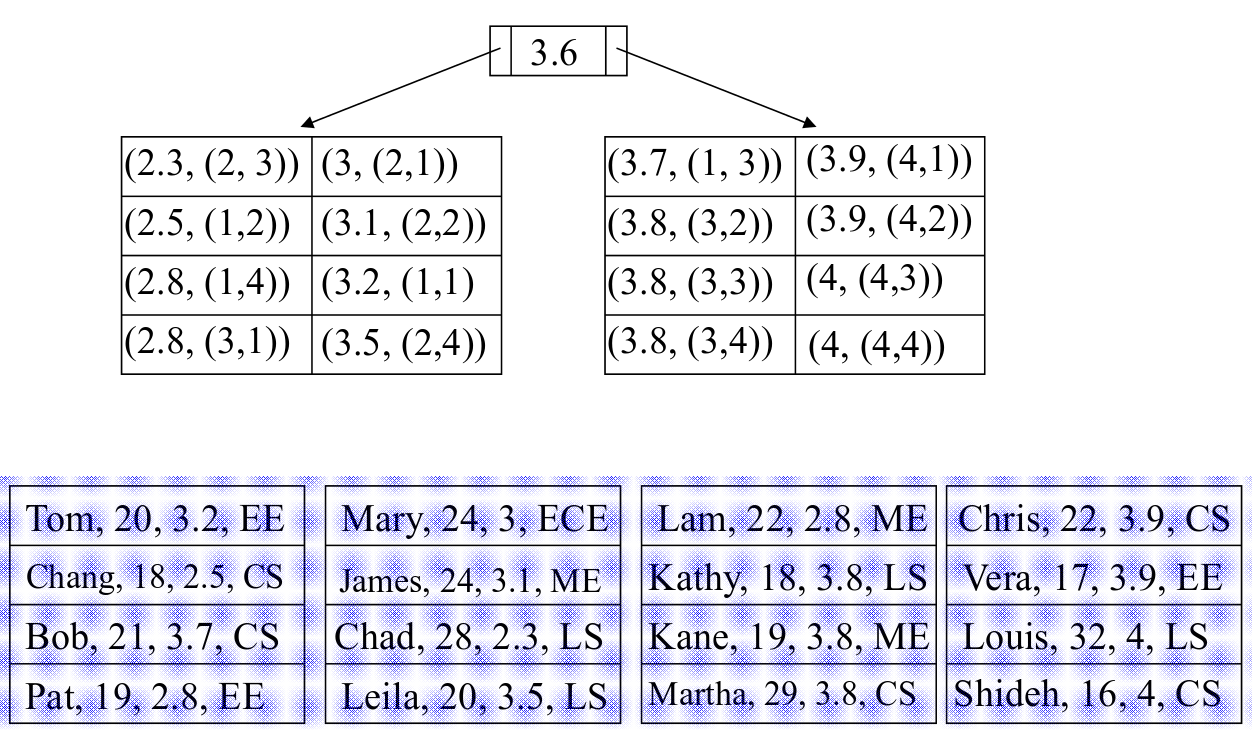
\includegraphics[width=0.33\textwidth]{BPTree}\end{figure}
\end{itemize}



\paragraph{Index --- kd-tree}
\begin{itemize}
	\item B+T löst Bar-Problem nicht wirklich
	\item kd-tree: Splitting für eine Dimension nach der anderen, dann wieder von vorne
	\item Beispiel: Vier Split-Dimensionen
\end{itemize}
\begin{figure}[H]\centering\label{KDTree}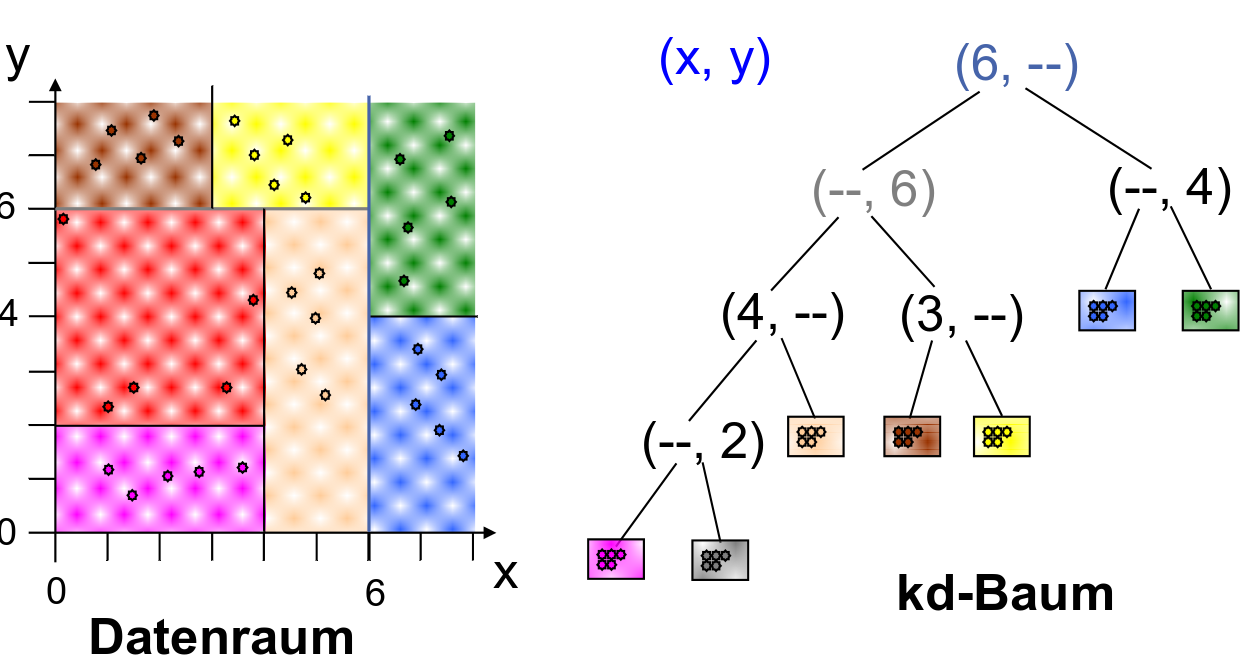
\includegraphics[width=0.33\textwidth]{KDTree}\end{figure}

\paragraph{kd-tree --- k-NN}
\begin{itemize}
	\item k-NN (= \emph{k-next-neighbour}) := Abstand des \( k \)-nächsten Nachbarn
	\item Es müssen nur ein paar kd-Baum-Regionen inspiziert werden, um Resultat zu ermitteln (Abstand zu Region ist untere Schranke)
	\item \textbf{Implementierung}: Priority Queue (Datenobjekte/Baumknoten, sortiert nach Abstand zum Anfragepunkt) initialisiert mit Wurzelknoten; Vorderstes Objekt aufspalten und Teilobjekte einfügen; Ende wenn Punkt vorne in Queue
	\item Hier: Baum unbalanciert, Balancierung in Realität für mehrdimensionale Daten
\end{itemize}

\paragraph{Outlier}
\begin{itemize}
	\item Element des Datenbestands, das in bestimmter Hinsicht erheblich vom restlichen Datenbestand abweicht
	\item Mögliche Definition: \\*
		Objekt \( O \), das in Datenbestand \( T \) enthalten ist ist ein DB(\( p \), \( D \))-Outlier, wenn der Abstand von \( O \) zu mindestens \( p \) Prozent der Objekte in \( T \) größer ist als \( D \).
	\item \textbf{Beispiel}: \( O \) ist Outlier, wenn \( p=0.6 \), da dann mehr als \( 60\% \) der Datenobjekte außerhalb des Kreises liegen
\end{itemize}
\begin{figure}[H]\centering\label{Outlier}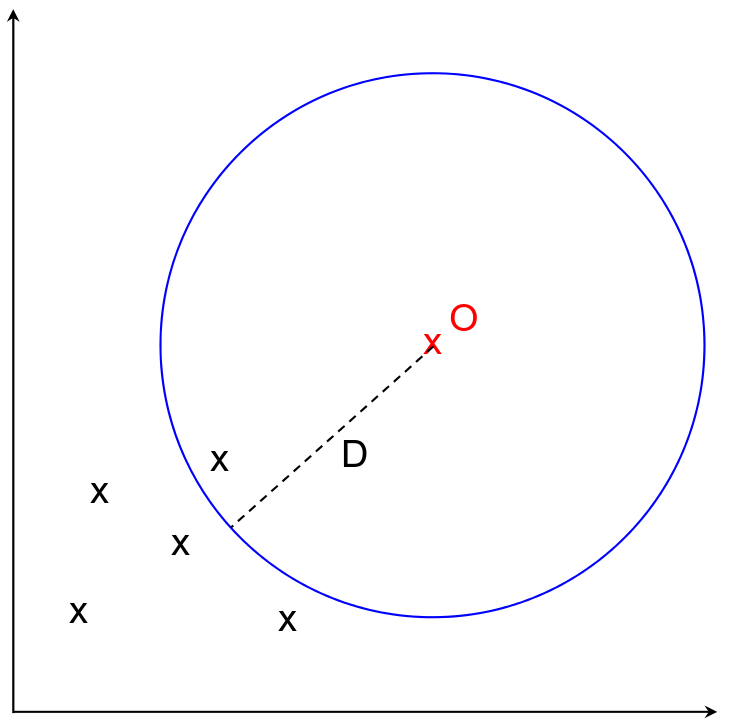
\includegraphics[width=.2\linewidth]{Outlier}\end{figure}

\paragraph{Outlier --- Index-basiert}
\begin{itemize}
	\item Punkt ist kein Outlier, wenn k-Abstand < D mit $k = N * (1 - p) - 1$
	\item Für jeden Punkt:\\*
		k-NN Query, dabei stoppen sobald größte noch mögliche k-NN Distanz < D  (Baumknoten mit k Objekten und größter Distanz < D)
	\item Viele weitere Ansätze, z.B. \\*
		\textbf{Clustering}: Liefert Outlier als Beiprodukt
\end{itemize}



\paragraph{Clustering --- Beispiel Customer Segmentation}
\begin{itemize}
	\item Große Kundendatenbank mit Eigenschaften und Käufen
	\item Gesucht: Gruppen von Kunden mit ähnlichem Verhalten finden
\end{itemize}

\paragraph{Clustering --- DBSCAN}
\begin{itemize}
	\item \textbf{Dichte}: Anzahl Objekte pro Volumeneinheit
	\item \textbf{Dichtes Objekt}: mindestens \( x \) andere Objekte in Kugel um Objekt mit Radius \( \epsilon \) (A)
	\item \textbf{Dichte-erreichbares Objekt}: Objekt in \( \epsilon \)-Umgebung eines dichten Objekts, das selbst nicht dicht ist (B, C) \\*
		Clusterrand, Zuordnung zu Clustern ist nichtdeterministisch
	\item \textbf{Rauschen} (\emph{Noise}): Objekte, die von keinem dichten Objekt erreicht werden können (N)
\end{itemize}
\begin{figure}[H]\centering\label{DBSCAN}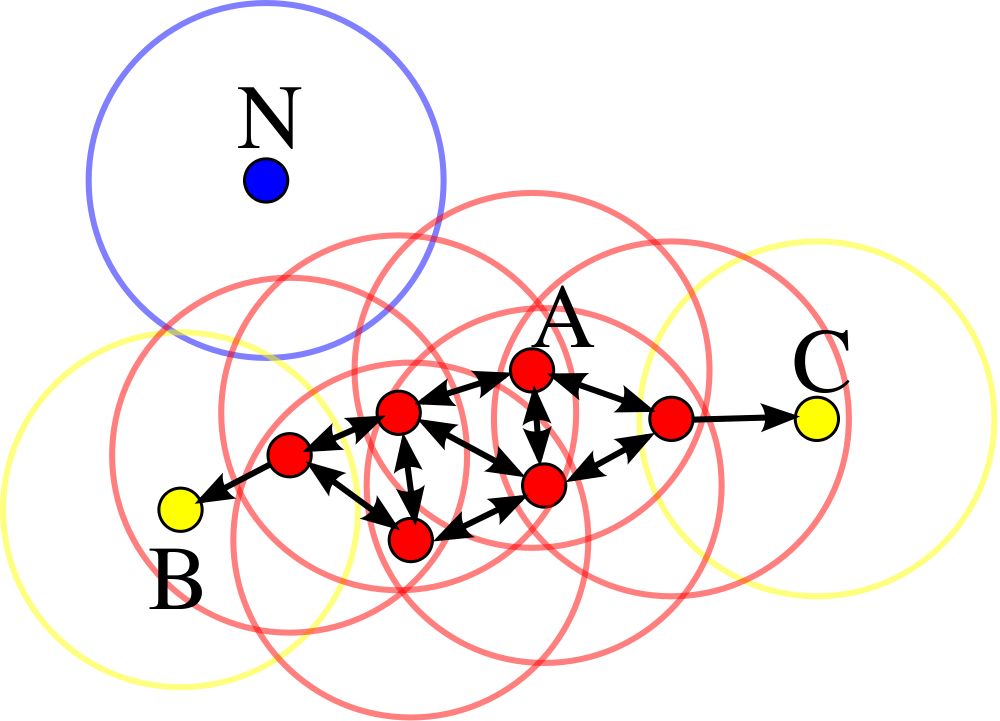
\includegraphics[width=0.2\textwidth]{DBSCAN}\end{figure}

\paragraph{DBSCAN --- Eigenschaften}
\begin{itemize}
	\item \textbf{Komplexität}: Lineare, wenn \( \epsilon \)-Umgebungen vorberechnet wurden (oder mit räumlichem Index in konstanter Zeit bestimmt werden können) \\* \( \leadsto \) mehrdimensionale Indexstruktur sehr sinnvoll
	\item Rauschen liefert \emph{mögliche} Outlier (DBSCAN erstellt Vorauswahl)
\end{itemize}

\paragraph{Hochdimensionale Datenräume --- Anomalien}
\begin{itemize}
	\item Curse of dimensionality
	\item \textbf{Sparsity}: Raum ist nur dünn mit Punkten besetzt
	\item Hierarchische Datenstrukturen ineffektiv: Es müssen immer alle Blätter betrachtet werden
	\item Keine echten Outlier: bei sehr, sehr vielen Dimensionen ist Abstand zweier Datenobjekte fast gleich dem zweier anderer \( \leadsto \) Outlier-Algorithmen liefern mehr oder weniger zufälliges Objekt
	\item \( \leadsto \) nur erfolgsversprechende Teilräume nach Ausreißern absuchen
	\item Interessante Cluster sind i.d.R. nicht Cluster in allen Dimensionen
\end{itemize}

\paragraph{Outlier --- im Höherdimensionalen}
\begin{itemize}
	\item Outlier erscheinen als solche nur in Teilräumen
	\item Manche Teilräume ausreißerfrei
	\item Unterschiedlichdimensionale Teilräume enthalten Ausreißer
	\item trivial vs. nichttrivial: \\*
		- \emph{trivial}: Objekt ist in Teilraum bereits Ausreißer \\*
		- \emph{nichttrivial}: Gegenteil
	\item \( \leadsto \) Maß für Teilraumrelevanz --- wie findet man relevante TR?
\end{itemize}

\paragraph{Subspace Search}
\begin{itemize}
	\item Exponentiell viele Teilräume \( P(A) \)
	\item Auswahl relevanter Teilräume \( RS \subset P(A) \)
\end{itemize}

\paragraph{HiCS --- Prinzip}
\begin{itemize}
	\item Attribute korrelieren nicht \( \leadsto \) Outlier in diesem Raum tendenziell eher trivial
	\item \textbf{Idee}: Suche nach Verletzung statistischer Unabhängigkeit \\* (= \emph{Kontrast})
\end{itemize}

\begin{fragen}
	\item Warum kann man räumliche Anfragen nicht ohne Weiteres auswerten, wenn man für jede Dimension separat einen B-Baum angelegt hat?
	\item Wie funktioniert der Algorithmus für die Suche nach den \( k \) nächsten Nachbarn mit Bäumen wie dem kd-Baum?
	\item Warum werden bei der NN-Suche nur genau die Knoten inspiziert, deren Zonen die NN-Kugel überlappen?
	\item Was ist ein Outlier?
	\item Was ist ein Zusammenhang zwischen \( k \)-NN-Suche mit Bäumen wie dem kd-Baum und Outlier-Berechnung?
	\item Warum ist die Zuordnung Dichte-erreichbarer Punkte mit DBSCAN nichtdeterministisch?
	\item Warum sind hierarchische Datenstrukturen in hochdimensionalen Merkmalsräumen für die \( k \)-NN-Suche nicht das Mittel der Wahl?
	\item Was bedeutet \emph{Subspace Search}?
	\item Geben Sie die Unterscheidung zwischen trivialen und nichttrivialen Outliern aus der Vorlesung wieder.
	\item Was genau bedeutet \emph{Kontrast} im Kontext von HiCS?
\end{fragen}